\chapter{Nutzerstudie}
\label{chap:evaluation}
\todo{Fragebögen, Flyer, Infobögen etc. in Anhang.}
Wie bereits in \autoref{chap:related_work} erwähnt ist ein Nachteil von 2D-Karten, dass durch das Fehlen einer Dimension zum Abgleich mit der Umgebung ein gewisser mentaler Aufwand notwendig ist.
Die 2D-Karte stellt eine Abstraktion der Umgebung dar, wodurch Informationen verloren gehen.

Der Zweck dieser Nutzerstudie ist zu überprüfen, ob sich bei den Probanden durch die 3D-Megamap ein räumliches Verständnis aufbaut, welches gegenüber der 2D-Karte zu einer performanteren und effizienteren Orientierung führt.
Unter Performanz und Effizienz wird in diesem Sinne verstanden, dass die Fehlerquote und die Zeit zum Einschätzen von Richtungen zu Orten in der Umgebung niedriger sind, als bei der 2D-Variante.
Zudem sollen die subjektiven Eindrücke und Präferenzen der Probanden von den unterschiedlichen Kartenvarianten ermittelt werden.
Für zukünftige Arbeiten werden außerdem Verbesserungsvorschläge und Ansichten über das Potential der Megamap gesammelt.

\section{Aufbau}
Das Experiment wurde im Laborraum 5220 (MZH Ebene 5) der Arbeitsgruppe Human-Computer Interaction an der Universität Bremen durchgeführt.
Für die Präsentation der virtuellen Umgebung wurde die HTC Vive mit zwei Basisstationen eingesetzt.
Der getrackte Bereich zwischen den Basisstationen umfasste ca. \SIrange{0}{0}{\metre}.\todo{Tatsächliche Zahlen einsetzen.}
Die Bilddaten wurden von einem PC mit einer \emph{NVidia~GTX~1080~Ti} Grafikkarte und einem \emph{AMD~Ryzen~7~1800X} Prozessor gerendert.
Übertragen wurden die Bilddaten an das HMD mit dem \emph{VIVE~Wireless~Adapter} \parencite{HTCCorporation2018b}.
Die Fragebögen wurden über \emph{Google Forms} erstellt und ausgefüllt (siehe \autoref{appendix:study_material}).
Hierfür wurde ein separater Laptop bereitgestellt.

\section{Konditionen und Aufgaben}
\label{sec:conditions_and_tasks}
Für die Nutzerstudie wurden drei unterschiedliche Konditionen getestet:
\begin{itemize}
    \item $3D_l$ (\emph{low)}: Die 3D-Megamap wird mit einer Skalierung von \SI{6}{\percent} (relativ zur Umgebung) und \SI{25}{\cm} über dem Boden angezeigt.
    Diese Kondition entspricht am ehesten der Megamap aus TCTD. 
    \item $3D_h$ (\emph{high}): Die 3D-Megamap wird mit einer Skalierung von \SI{6}{\percent} (relativ zur Umgebung) und \SI{1}{\metre} unterhalb der HMD-Position angezeigt.
    Dabei wird die Höhe nur beim Aufrufen der Karte berechnet.
    Danach bleibt die Höhe fix.
    Diese Kondition wird getestet, um zu ermitteln, wie sich die Höhe der Megamap vom Boden auf die Nutzung auswirkt (insbesondere unter dem Aspekt, dass durch die Darstellung in 3D Verdeckungen durch die Wände der Räume auftreten können).
    \item $2D$: Eine 2D-Karte wird senkrecht an der Wand vor dem Nutzer angezeigt.
    Auch die 2D-Karte hat eine Skalierung von \SI{6}{\percent} (relativ zur Umgebung).
    Die Karte ist so an der Wand platziert, dass sie nicht von anderen Wänden oder der Decke und dem Fußboden geschnitten wird.
\end{itemize}
\todo{Screenshots der Konditionen einfügen.}

Jede Kondition wurde über 6~Iterationen (\emph{Tasks}) $T_0, \dots, T_5$ wiederholt.
\todo{Bild für Megamap Varianten} Dabei wurde in jeder Iteration eine andere Indoor-Karte für die Megamap verwendet, um einen Lerneffekt für die Kartenlayouts zu minimieren.
Damit die Konditionen vergleichbar bleiben, wurde jede Karte einmal jeder Kondition unterzogen.
Das heißt, die Probanden durchliefen insgesamt 18~Iterationen, wobei sechs unterschiedliche Karten jeweils dreimal eingesetzt wurden.
Die Reihenfolge der Iterationen innerhalb einer Kondition war zufällig bestimmt, wobei darauf geachtet wurde, dass bei einem Wechsel der Konditionen die gleiche Karte nicht zweimal aufeinander folgte.

Um die Auswirkungen der jeweiligen Kondition auf die mentale räumliche Vorstellung des Probanden von der Umgebung zu testen, wurden eine Suchaufgabe und eine Richtungsschätzung in den Prototypen integriert.

Für die Suchaufgabe wurden auf der jeweiligen Megamap in sieben räumen Bälle platziert.
Die Probanden mussten dann den Raum suchen, der die meisten Bälle enthält und diesen mit dem VIVE Controller und dem virtuellen Laserpointer auswählen.
Jede Megamap hatte genau einen Zielraum, welcher zufällig zwischen sieben und zehn Bällen enthielt.
Die anderen Räume enthielten mindestens fünf Bälle und garantiert weniger als der Zielraum.
Jede der sechs Indoor-Karten hatte denselben Zielraum in allen drei Konditionen.
Dies wurde entschieden, damit die Karten über Konditionen hinweg vergleichbar bleiben.
Wäre immer ein anderer Zielraum gewählt worden, wäre der Schwierigkeitsgrad des Findens zwischen den Konditionen unter Umständen verschieden gewesen, obwohl die Karte die gleiche wäre.

Für den Fall, dass ein Proband einen falschen Raum auswählt, würde dieser rot eingefärbt werden.
Der Proband müsste dann die Suche nach dem Zielraum fortfahren.
Dieser Fall trat über alle Probanden hinweg außerhalb des Tutorials nur ein einziges Mal auf.

Die Probanden mussten sich anhand der Megamap die Richtung vom virtuellen Laborraum zum Zielraum (horizontal und vertikal zentriert) merken.
Sobald sie den Zielraum auswählten, wurde die Megamap ausgeblendet.
Mit dem virtuellen Laserpointer sollten die Probanden dann möglichst mittig auf den Zielraum \emph{in ihrer Umgebung} zeigen.
Durch Betätigen des Triggers konnte der Laserpointer \enquote{eingefroren} werden, um die Richtung entweder zu korrigieren oder zu akzeptieren.
Wenn die Richtung akzeptiert wurde, startete die nächste Iteration.

Damit die Probanden beim Suchen auf einer Karte immer die gleiche Startposition und Blickrichtung hatten wie in den anderen Konditionen, wurde vor der Suchaufgabe ein \emph{User Setup} implementiert.
Die Probanden mussten sich dabei auf eine festgelegte Zielposition stellen und für zwei Sekunden auf ein Ziel an der Wand schauen.
Die beiden Zielpositionen waren von der jeweiligen Karte abhängig, bleiben jedoch für eine Karte über die Konditionen hinweg gleich.
So wurde sichergestellt, dass die Ausgangsbedingungen für die Suche auf der Karte in jeder Kondition gleich bleiben.

Ebenso wurde das User Setup zwischen der Suche und der Richtungsschätzung implementiert.
Ohne diesen Zwischenschritt hätten die Probanden in den 3D-Konditionen einfach den Laserpointer vom Raum auf der Karte anheben müssen, um die korrekte Richtung zu schätzen.
Durch das User Setup wurde eine Ablenkung erzeugt, welche diesen Vorteil der 3D-Konditionen gegenüber der 2D-Kondition minimieren soll.

\section{Ablauf}
Für einen Test wurden \num{45}~Minuten angesetzt.

Zuerst bekamen die Probanden Hintergrundinformationen zu der Nutzerstudie.
Unter anderem wurde erklärt, dass eine neuartige 3D-Darstellung von Indoor-Karten für MR/VR getestet wird und dass verschiedene Varianten getestet würden.
Mit einem Informationsbogen wurden die Probanden über die Details, den Ablauf sowie die gesammelten Daten der Nutzerstudie aufgeklärt.
Daraufhin unterschrieben die Probanden einen Zustimmungsbogen (siehe \autoref{appendix:study_material}).
Dabei willigten zur Teilnahme an der Studie sowie der Aufzeichnung ihres Blickfelds in der virtuellen Umgebung ein.
Die Probanden konnten frei entscheiden, ob zusätzlich eine Audioaufnahme der Gespräche während des Experiments aufgezeichnet wird.

Vor dem eigentlichen Test füllten die Probanden einen allgemeinen Fragebogen aus (siehe \autoref{appendix:study_material}).
Dieser enthielt Fragen zur Person (Alter, Geschlecht usw.) sowie Vorerfahrungen in VR/MR und mit Kartenanwendungen für Außen- und Innenbereiche. Der letzte Teil des Fragebogens ist die ins Deutsche übersetzte Santa~Barbara~Sense-of-Direction~Scale \parencite{Hegarty2002}, mit dem Probanden Selbstauskunft über ihren Orientierungssinn geben.
Die Bewertung wurde von einer 7-Punkte- auf eine 5-Punkte-Likert-Skala abgeändert, um mit den späteren Fragebögen einheitlich zu sein.

Den Probanden wurde danach das VR-Equipment (HMD und Batteriepack für den Wireless~Adapter) angelegt.
Sie fanden sich im virtuellen Laborraum wieder.
Die Probanden wurden kurz in der Bedienung des VIVE Controllers und der Bewegung im Raum innerhalb der Play Area unterrichtet.
Sie wurden darauf hingewiesen, dass an einer der Wände ein Bildschirm hängt, der ihnen den nächsten Aufgabenschritt in Textform anzeigt, sollten sie den Ablauf vergessen.
Die Probanden konnten auch jederzeit während des Experiments Fragen an den Versuchsleiter stellen.

Es folgte ein Tutorial, bei dem die Probanden die zuvor beschriebenen Aufgaben (User~Setup --- Suche --- User~Setup --- Zeigen) in einer Tutorialkondition durchliefen (\SI{40}{\cm} Kartenhöhe vom Boden bei \SI{4}{\percent} Skalierung).
Zuerst wurde die 3D-Megamap gezeigt, danach die 2D-Kondition.
Die Probanden konnten entscheiden, ob sie das Tutorial wiederholen oder fortfahren wollen.
Zu diesem Zeitpunkt wurde die Bildschirmaufnahme (und ggf. die Audioaufnahme) gestartet.

Nach dem Tutorial durchliefen die Probanden die Konditionen und Aufgaben, wie sie in \autoref{sec:conditions_and_tasks} beschrieben sind.
Nach jeder Kondition setzten die Probanden das HMD ab und füllten am Laptop einen Fragebogen zur zuletzt gestesteten Kartenvariante aus (siehe \autoref{appendix:study_material}).
Die Fragebögen basieren auf der \emph{System~Usability~Scale}, wurden jedoch für das Anwendungsgebiet von Karten angepasst.
Die Bewertung der einzelnen Aussagen erfolgte über eine 5-Punkte-Likert-Skala.

Nach Abschluss des letzten Fragebogens wurde mit den Probanden ein kurzes (5--10 Minuten) Leitfadeninterview geführt.
Unter anderem beantworteten die Probanden Fragen zu ihrer präferierten Kartenvariante fürs Suchen und Richtungsschätzen, ihr Vorgehen beim Suchen sowie Verbesserungsvorschlägen.
Die Probanden wurden auch befragt, ob sie sich einen Einsatz von 3D-Megamaps mit MR-HMDs in der realen Welt sowohl in Innen- als auch Außenbereichen vorstellen können.

\section{Testgruppe}
An der Nutzerstudie nahmen 15~Personen teil ($user\_0, \dots, user\_14$), davon 10~männlich und 5~weiblich.
Die Probanden befanden sich in einem Altersbereich von ?? bis ?? Jahren.
Vier der Probanden sind Brillenträger von denen zwei die Brille aus Bequemlichkeitsgründen während des Tests abnahmen.
Zwei der Probanden sprachen Englisch und füllten ins Englische übersetzte Versionen der Fragebögen aus.
Die Muttersprache aller anderen Probanden ist Deutsch.
Keiner der Probanden war in die Inhalte der Masterarbeit oder der Nutzerstudie eingeweiht.

Die Probanden wurden durch an der Universität ausgehängte Flyer (siehe \autoref{appendix:study_material}), den Mailverteiler des Fachbereichs~3 und über die Arbeitsgruppe Human-Computer~Interaction rekrutiert.
Einige Probanden wurden außerdem durch persönlichen Kontakt mit dem Versuchsleiter angeworben.
Für die Teilnahme wurden den Probanden Snacks und Getränke angeboten.
Eine finanzielle Aufwandsentschädigung gab es nicht.

Bei $user_4$ kam es während der ersten Kondition ($3D_h$) zu einem PC-Absturz, der aus einer Inkompatibilität zwischen dem Ryzen-Prozessor und dem VIVE Wireless Adapter resultiert \parencite{HTCCorporation2018c}.
Auch bei einem erneuten Start des Experiments kam es in der Kondition $3D_h$ zum Absturz.
Daraufhin wurde der Test abgebrochen.
Der Proband erschien wenige Tage später und führte das Experiment erneut ohne Absturz durch.
Es wird darauf hingewiesen, dass dieser Nutzer durch die vorige begrenzte Teilnahme für seinen Durchlauf mehr Vorkenntnisse hatte, als die anderen Probanden.

\section{Datenerhebung}
Neben den Antworten aus den Fragebögen wird das Sichtfeld der Proband in der virtuellen Welt aufgezeichnet (und ggf. eine Audioaufnahme des Gesagten).

Zum Vergleich der Performanz von 2D und 3D wird beim Richtungsschätzen die horizontale und vertikale Abweichung von der \enquote{korrekten} Richtung berechnet.
Als korrekte Richtung gilt der Vektor von der Controllerspitze zum Zentrum des Zielraums in der Umgebung.
Die horizontale und vertikale Abweichung ergeben sich aus den jeweiligen Winkeln zwischen der vom Probanden bestätigten Richtung und der korrekten Richtung.

Zum Vergleich der Effizienz werden diverse Zeitmessungen durchgeführt.
Zum einen wird die Zeit gemessen, die Probanden zum Finden des Zielraums benötigen.
Zum anderen wird die Zeit gemessen, bis Probanden die geschätzte Richtung bestätigt haben.
So sollen Aussagen über die Zuversicht der Probanden ihrer Schätzung getroffen werden.

Darüber hinaus werden kontinuierlich die Positionen und Rotationen des HMDs und des Controllers aufgezeichnet.

\section{Ergebnisse}


\subsection{Santa-Barbara Sense-of-Direction Skala}
Vor dem eigentlichen Test füllten Probanden einen Fragebogen nach der SBSOD Skala aus.
Dieser liefert eine Wertung des vom Probanden selbst wahrgenommenen Orientierungssinn.
Zur Auswertung werden die positiv formulierten Elemente invertiert bewertet.
Anschließend wird der Mittelwert über die individuellen Bewertungen berechnet.
Der Mittelwert entspricht der SBSOD-Wertung \parencite{Hegarty2002}.
\autoref{fig:sbsod} stellt das Ergebnis grafisch dar.
Von den 14 Probanden erreichten 12 (\SI{85,71}{\percent}) einen Wert über 3 (\enquote{neutral}).
Im Schnitt wurde eine Bewertung von 3,38 ($\pm$ 0,41) erzielt.
Der höchste erreichte Wert ist 4,07, der niedrigste Wert ist 2,67.
\begin{figure}
    \centering
    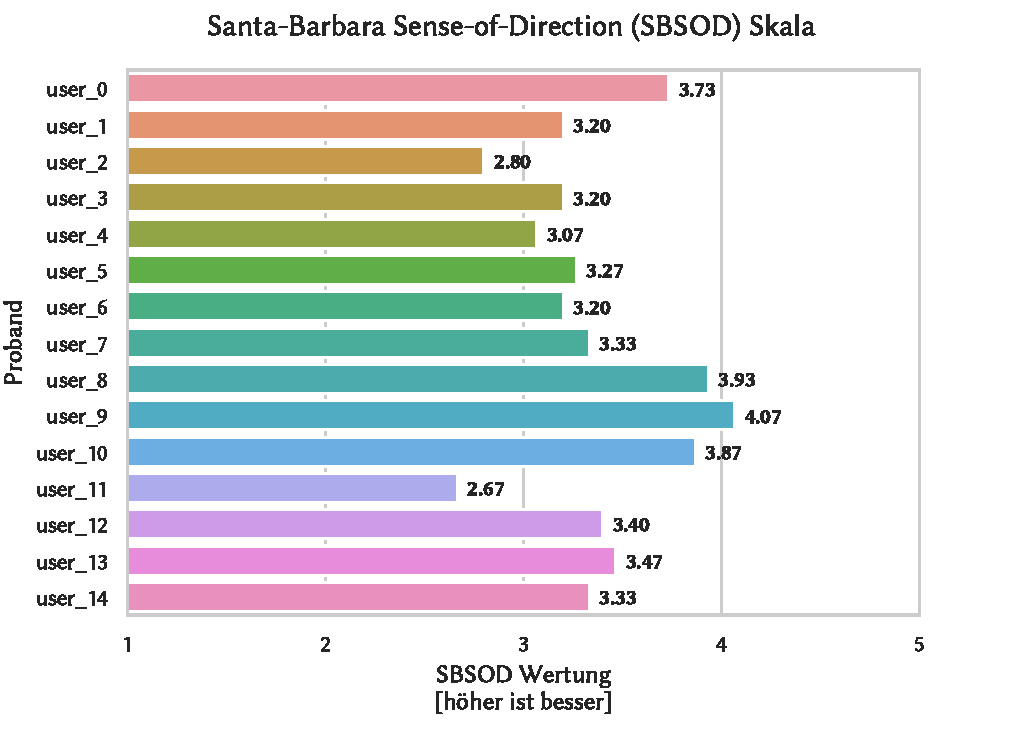
\includegraphics[trim={2cm, 0, 2cm, 0}, clip, width=\linewidth]{figures/analysis/sbsod}
    \caption{text}
    \label{fig:sbsod}
\end{figure}

\subsection{Effektivität und Effizienz bei Raumsuche}
\subsubsection*{Suchzeit}
\label{ssec:searchtime}

\begin{table}
    \centering
    \caption{Mittelwert $\mu$ und Standardabweichung $\sigma$ der Suchzeit über alle Karten je Kondition.}
    \label{tab:searchtime_overview}
    \begin{tabular}{rccc}
        \toprule
        {} & \multicolumn{3}{c}{Suchzeit [\SI{}{\second}]} \\
        {} &          $3D_l$ &          $3D_h$ &          $2D$ \\
        \midrule
        $\mu$    &  $\num{27.44}$     &  $\num{28.84}$     &  $\num{18.31}$ \\
        $\sigma$ &  $\pm \num{13.39}$ &  $\pm \num{10.08}$ &   $\pm \num{9.3}$ \\
        \bottomrule
    \end{tabular}
\end{table}

\autoref{tab:searchtime_overview} zeigt eine Übersicht der Suchzeit nach den Zielräumen zwischen den einzelnen Konditionen.
Da die Stichprobenverteilungen der beobachteten Zeiten nicht-normalverteilt ist (wie in \autoref{fig:searchtime_distributions} zu sehen ist), werden nicht-parametrisierte Tests zur Bestimmung der Signifikanz angewendet.
Zwischen den drei Konditionen ist nach dem Friedman-Test ein signifikanter Unterschied festzustellen ($\chi^2(2) = \num{63.5}, p < 0.001$).
Ein paarweiser Wilcoxon-Vorzeichen-Rang-Test zwischen den einzelnen Konditionen zeigt, dass die Suche nach dem Zielraum in $2D$ ($\num{18.31} \pm \SI{9.3}{\second}$) signifikant schneller ist als in $3D_l$ ($\num{27.44} \pm \SI{13.39}{\second}, z=\num{-6.003}, p<\num{0.001}$) und $3D_h$ ($\num{28.84} \pm \SI{10.08}{\second}, z=\num{-7.136}, p<0.001$).
Der Unterschied bei der Suchzeit zwischen $3D_l$ und $3D_h$ ist jedoch nicht signifikant.
\begin{figure}
    \centering
    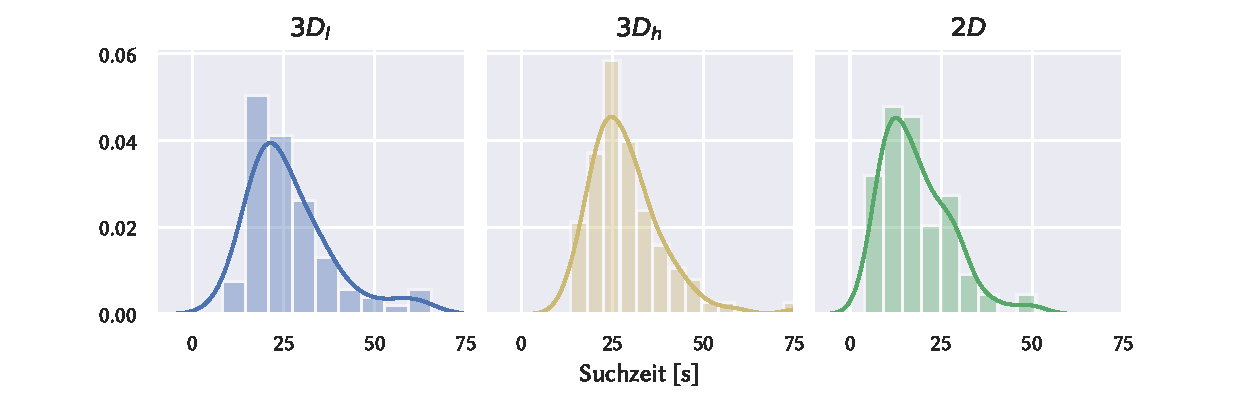
\includegraphics[width=\linewidth]{figures/analysis/searchtime_distributions}
    \caption{Stichprobenverteilung der beobachteten Suchzeit.}
    \label{fig:searchtime_distributions}
\end{figure}

Weiterhin stellt sich die Frage, ob ein \enquote{besserer} Orientierungssinn zu einer besseren Suchzeit führt.
\autoref{fig:correlation_time_sbsod} zeigt die durchschnittliche Suchzeit der Probanden in Bezug zu den ermittelten SBSOD-Werten aus \autoref{fig:sbsod}.
Für jede Kondition wird Spearmans Rangkorrelationskoeffizient zwischen der SBSOD-Wertung und der durchschnittlichen Suchzeit ermittel.
Die Tests weisen keinen signifikanten Zusammenhang der Variablen aus.
Probanden, die ihren Orientierungssinn besser einschätzen, sind demnach nicht zwingend schneller bei der Suche nach den Zielräumen.
\begin{figure}
    \centering
    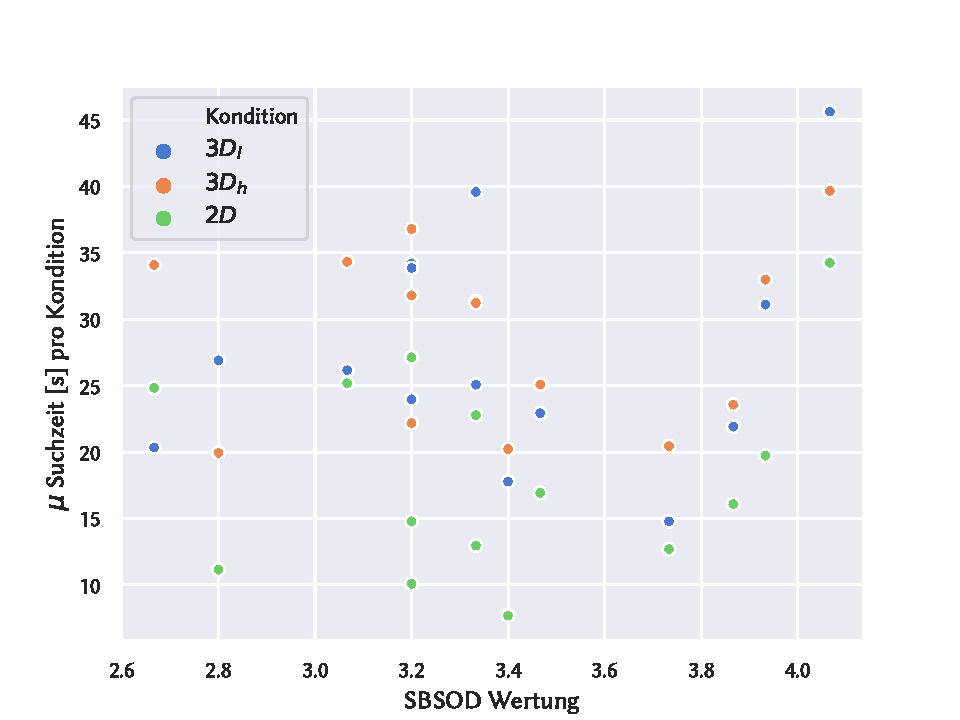
\includegraphics[width=\linewidth]{figures/analysis/correlation_time_sbsod_scatter}
    \caption{Scatterplot zur Überprüfung der Korrelation zwischen SBSOD Wertung und Suchzeit.}
    \label{fig:correlation_time_sbsod}
\end{figure}

\subsubsection*{Fehlerrate bei Raumauswahl}
Neben der Suchzeit wurde auch die Zahl der falsch ausgewählten Räume (die Nicht-Zielräume) gemessen.
Über die insgesamt 252 Suchaufgaben (14~Probanden $\times$ 3~Konditionen $\times$ 6~Karten) wurden in drei Fällen (\SI{1,19}{\percent}) vor dem Zielraum falsche Räume ausgewählt.
\autoref{tab:error_searching} zeigt eine Übersicht der entsprechenden Events.
Die Fehler treten jeweils in der ersten Kondition der getesteten Sequenz auf (jedoch nicht in der ersten Karte).
\begin{table}
    \centering
    \caption{Übersicht der Anzahl der falsch ausgewählten Räume währen der Suchaufgabe.}
    \label{tab:error_searching}
    \begin{tabular}{rccccc}\toprule
        Proband                  & Kondition               & Karte    & Suchzeit [\SI{}{\second}] & \# Fehler & Sequenz  \\\midrule
        user\_8                  & $3D_h$                  & Karte\_6 & $\SI{40,61}{\second}$     & 2         & $3D_h$--$3D_l$--$2D$ \\
        user\_9                  & $2D$                    & Karte\_5 & $\SI{38,4}{\second}$      & 1         & $2D$--$3D_l$--$3D_h$ \\\bottomrule
    \end{tabular}
\end{table}

\subsection{Performance und Effizient bei Richtungsschätzung}
\subsubsection*{Genauigkeit der Schätzung}
\autoref{fig:horizontal_offset} zeigt das Ergebnis der Richtungsschätzung.
Da die Abweichung sowohl in positiven Winkeln (Abweichung nach rechts) als auch negativen Winkeln (Abweichung nach links) gemessen wurde, werden hier die absoluten Werte der Abweichung analysiert.
Andernfalls würden die Werte sich bei der Mittelwertbildung gegenseitig aufheben.
Wie zu erkennen ist, liegen die Mittelwerte von $3D_l$~(7,79 $\pm$ \ang{7,22}), $3D_h$~(7,84 $\pm$ \ang{7,44}) und $2D$~(6,62 $\pm$ \ang{5,28}) nahe beieinander.
Der Friedman-Test kann keine signifikanten Unterschiede zwischen den Konditionen nachweisen.
\begin{figure}
    \centering
    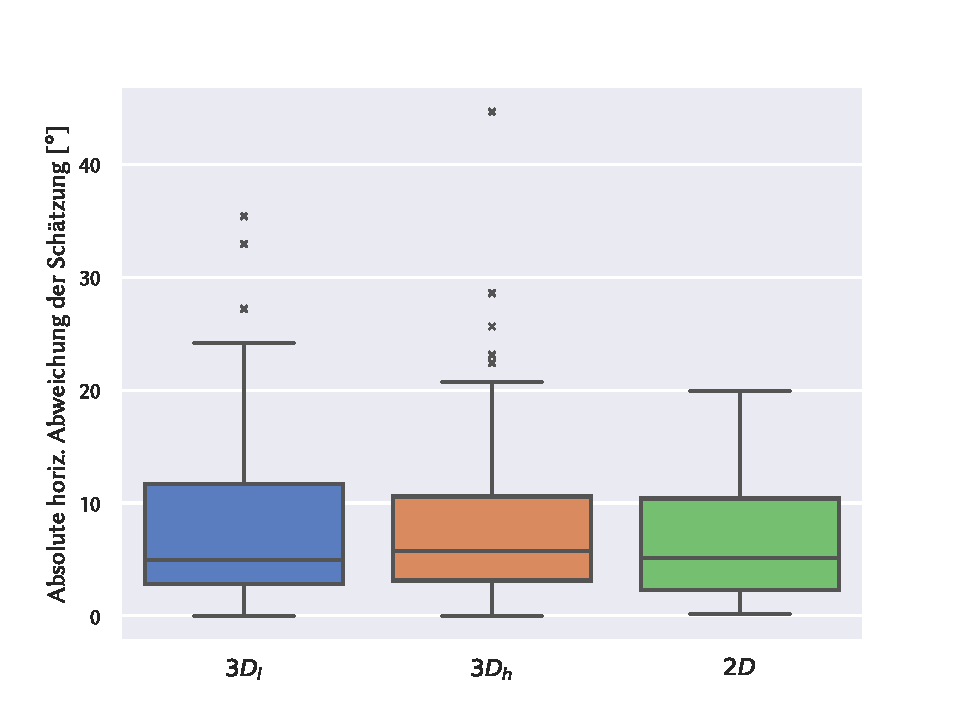
\includegraphics[height=0.45\textheight]{figures/analysis/horizontal_offset}
    \caption{Horizontale Abweichung in $\degree$ (Grad) bei der Richtungsschätzung von der tatsächlichen Linie zur Raummitte (ohne vertikale Abweichung).}
    \label{fig:horizontal_offset}
\end{figure}

Ein wesentlicher Aspekt, der die Genauigkeit der Schätzung beeinflusst, ist die Position des Zielraums auf der jeweiligen Karte.
\autoref{tab:herror_per_map} fasst die Mittelwerte und Standardabweichungen der absoluten horizontalen Abweichungen der einzelnen Karten zusammen.
\autoref{fig:horizontal_offset_per_map} zeigt die Unterschiede zwischen den Karten grafisch.
Es ist zu erkennen, dass vor allem die Abweichungen bei Karte 3 und 4 größer sind, als auf den anderen Karten.
Der Friedman-Test bestätigt signifikante Unterschiede zwischen den Karten ($\chi^2(6) = \num{39.755}, p < \num{0.001}$).
Die horizontale Abweichung bei Karte~3 ist signifikant größer als bei Karte~1 ($z = \num{-4,483}, p < \num{0,001}$), Karte~2 ($z = \num{-4,195}, p < \num{0,001}$), Karte~5 ($z = \num{-3,432}, p < \num{0,001}$) und Karte~6 ($z = \num{-3,37}, p < \num{0,001}$).
Auch die hohe Abweichung bei Karte~4 ist gegenüber Karte~1 ($z = \num{-3,782}, p < \num{0,001}$), Karte~2 ($z = \num{-3,395}, p < \num{0,001}$), Karte~5 ($z = \num{-2,044}, p < \num{0,05}$) und Karte~6 ($z = \num{-2,17}, p < \num{0,05}$) signifikant.
Weiterhin gibt es bei Karte~5 eine signifikant größere Abweichung als bei Karte~1 ($z = \num{-2,645}, p < \num{0,008}$), was durch die Ausreißer (siehe \autoref{fig:horizontal_offset_per_map}) begünstigt wird.
\begin{figure}[h!]
    \centering
    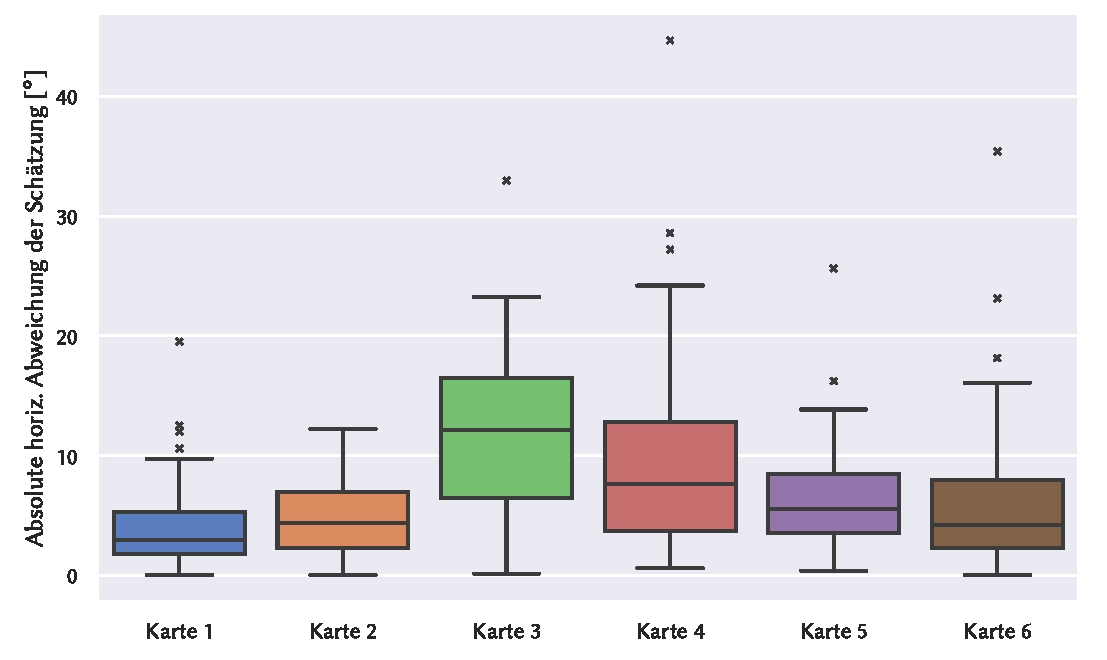
\includegraphics[width=0.75\linewidth]{figures/analysis/horizontal_offset_per_map}
    \caption{Absolute horizontale Abweichung in $\degree$ (Grad) bei der Richtungsschätzung pro Karte.}
    \label{fig:horizontal_offset_per_map}
\end{figure}%

\begin{table}[h!]
    \centering
    \caption{Mittelwert $\mu$ und Standardabweichung der absoluten horizontalen Abweichung pro Karte in $\degree$.}
    \label{tab:herror_per_map}
    \begin{tabular}{cccccc}\toprule
        Karte 1 & Karte 2 & Karte 3 & Karte 4 & Karte 5 & Karte 6 \\\midrule
        $\mu = \ang{4,44}$ & $\mu = \ang{4,96}$ & $\mu = \ang{11,75}$ & $\mu = \ang{10,19}$ & $\mu = \ang{6,62}$ & $\mu = \ang{6,55}$ \\
        $\pm \ang{4,03}$ & $\pm \ang{3,3}$ & $\pm \ang{6,98}$ & $\pm \ang{9,07}$ & $\pm \ang{4,94}$ & $\pm \ang{7,05}$ \\\bottomrule
    \end{tabular}
\end{table}

Wird der Unterschied zwischen der positiven und negativen horizontalen Abweichung mit einbezogen, ist eine Tendenz zu einem Ausschlag nach links (negativ) der horizontalen Abweichungen zu erkennen.
Von den insgesamt 252~Richtungsschätzungen weichen 158 (\SI{62,7}{\percent}) nach links ab.

\subsubsection*{Schätzungszeit}
Neben der Abweichung der Schätzung wurde auch die Zeit gemessen, welche die Probanden für die Abgabe der Schätzung benötigen.
\autoref{fig:pointing_time} visualisiert die erhobenen Daten.
In den meisten Iterationen (\SI{95,24}{\percent}) wurde die Richtungsschätzung innerhalb von 10~Sekunden bestätigt.

% TODO: Und weiter???

\begin{figure}
    \centering
    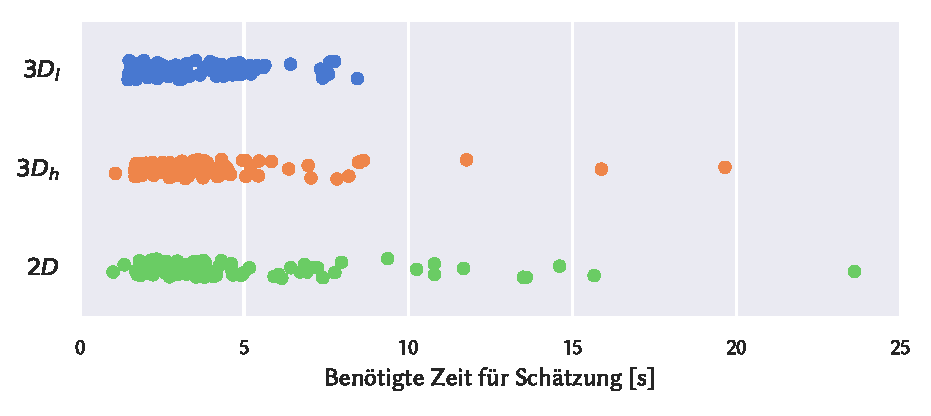
\includegraphics[width=\linewidth]{figures/analysis/pointing_time}
    \caption{Vergleich der Zeit (zwischen den Konditionen), die die Probanden für die Abgabe einer Richtungsschätzung benötigten.}
    \label{fig:pointing_time}
\end{figure}

Einer der Gründe für die Messung der Schätzzeit war es, die Korrelation zur resultierenden horizontalen Abweichung zu testen.
Die Überlegung ist, dass Probanden, die sich mehr Zeit für die Schätzung der Richtung nehmen, präziser sind.
\autoref{fig:pointing_time_vs_error} zeigt die absolute horizontale Abweichung in Bezug zur benötigten Schätzzeit.
Weder grafisch, noch doch Anwendung des Spearman-Tests, ist eine Korrelation zwischen den beiden Variablen erkennbar.
Da die meisten Probanden ihre Schätzung innerhalb der ersten 10~Sekunden abgegeben haben, sind für den Zeitraum \emph{nach} 10~Sekunden zu wenig Messungen vorhanden, um eine zuverlässige Aussage über eine potentielle Korrelation treffen zu können.
\begin{figure}
    \centering
    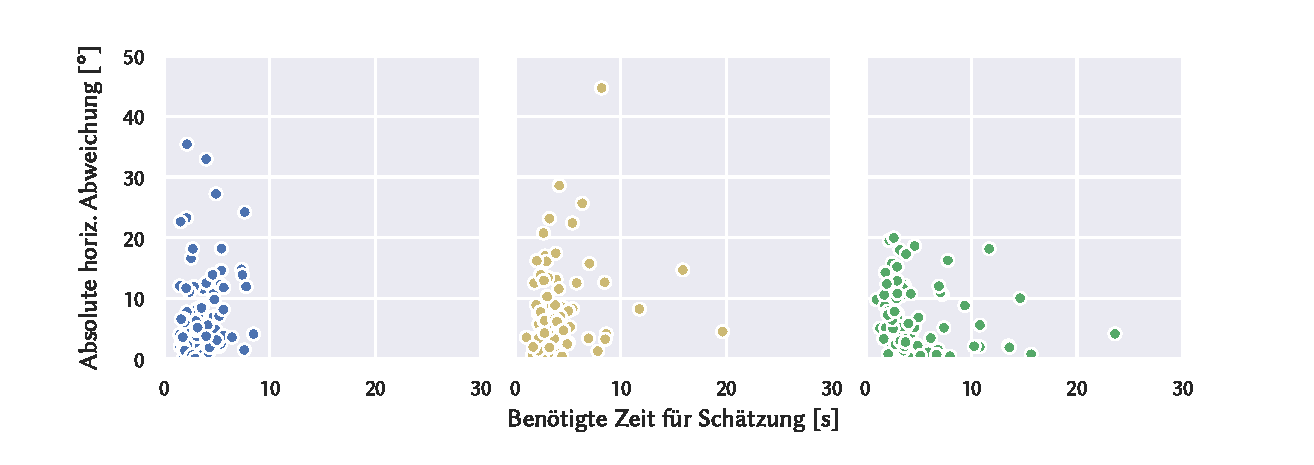
\includegraphics[width=\linewidth]{figures/analysis/pointing_time_vs_error}
    \caption{Plot der Schätzungszeit gegen die absolute horizontale Abweichung. %
    Eine Korrelation ist nicht erkennbar.}
    \label{fig:pointing_time_vs_error}
\end{figure}

\subsection{Fragebögen zur Nutzungsfreundlichkeit}

\begin{figure}
    \centering
    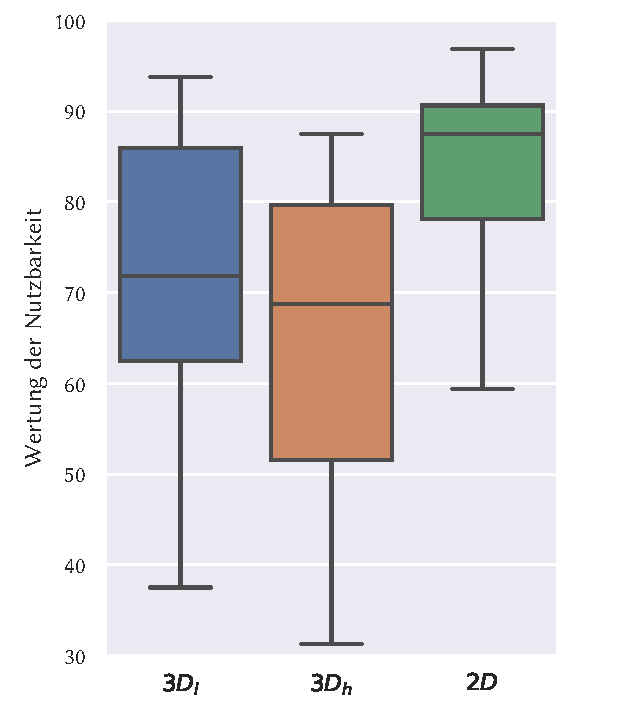
\includegraphics[width=\linewidth]{figures/analysis/usability}
    \caption{text}
    \label{fig:usability}
\end{figure}

\subsection{Präferenz der Probanden aus Interview}

\section{Diskussion der Ergebnisse}

%
\cleardoublepage
